\documentclass{standalone}
\usepackage{amsmath}
\usepackage{pgf,tikz}
\usepackage{mathrsfs}
\usetikzlibrary{arrows}
\pagestyle{empty}
\begin{document}

	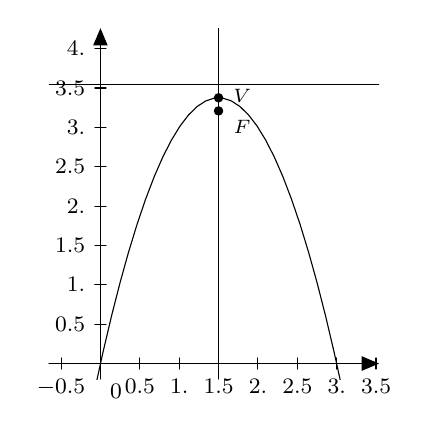
\begin{tikzpicture}[line cap=round,line join=round,>=triangle 45,x=1.0cm,y=1.0cm]
	\draw[->,color=black] (-0.6545542164564786,0.) -- (3.537612064685066,0.);
	\foreach \x in {-0.5,0.5,1.,1.5,2.,2.5,3.,3.5}
	\draw[shift={(\x,0)},color=black] (0pt,2pt) -- (0pt,-2pt) node[below] {\footnotesize $\x$};
	\draw[->,color=black] (0.,-0.1974866492503101) -- (0.,4.258522264970048);
	\foreach \y in {,0.5,1.,1.5,2.,2.5,3.,3.5,4.}
	\draw[shift={(0,\y)},color=black] (2pt,0pt) -- (-2pt,0pt) node[left] {\footnotesize $\y$};
	\draw[color=black] (0pt,-10pt) node[right] {\footnotesize $0$};
	\clip(-0.6545542164564786,-0.1974866492503101) rectangle (3.537612064685066,4.258522264970048);
	\draw (1.5,-0.1974866492503101) -- (1.5,4.258522264970048);
	\draw [samples=50,rotate around={-180.:(1.5,3.375)},xshift=1.5cm,yshift=3.375cm,domain=-2.6666666666666665:2.6666666666666665)] plot (\x,{(\x)^2/2/0.3333333333333333});
	\draw [domain=-0.6545542164564786:3.537612064685066] plot(\x,{(--3.5416666666666665-0.*\x)/1.});
	\begin{scriptsize}
	%\draw[color=black] (2.042503810571648,3.8383284419185664) node {$Asse$};
	\draw [fill=black] (1.5,3.375) circle (1.5pt);
	\draw[color=black] (1.8,3.4) node {$V$};
	\draw [fill=black] (1.5,3.2083333333333335) circle (1.5pt);
	\draw[color=black] (1.8,3) node {$F$};
	%\draw[color=black] (0.7623784426706169,3.447450466986956) node {$Direttrice$};
	\end{scriptsize}
	\end{tikzpicture}
\end{document}